%%%%%%%%%%%%%%%%%%%%%%%%%%%%%%%%%%%%%%%%%%%%%%%%%%%%%%%%%%%%%%%%%%%%%%%%%%%%%%%%
%                     Bachelor thesis template 
%						 Science Faculty 
%								at 
%			National Autonomous University of Mexico (UNAM)
%%%%%%%%%%%%%%%%%%%%%%%%%%%%%%%%%%%%%%%%%%%%%%%%%%%%%%%%%%%%%%%%%%%%%%%%%%%%%%%%
% based on Harish Bhanderi's PhD/MPhil template, then Uni Cambridge
% http://www-h.eng.cam.ac.uk/help/tpl/textprocessing/ThesisStyle/
% corrected and extended in 2007 by Jakob Suckale, then MPI-iCBG PhD programme
% and made available through OpenWetWare.org - the free biology wiki
%
%                     Under GNU License v3
%
% Adapted for the Engineering School at UNAM by Jesús Velázquez y Marco Ruiz
% Then, adapter fot he Science Faculty at UNAM by Jonathan Urrutia
%
%
%
% All used packages are found in  
%
%					./Latex/Classes/PhDthesisPSnPDF.cls
%
% within this las documments there are some lines to be UnCommented for a printed or a digital version of the output file:
%
%			line 184
%			lines 231-261
%
%	Since this is a template for a thesis made at UNAM (Mexico) the titles may be in spaninish but within PhDthesisPSnPDF.cls it can be change
%

\documentclass[11pt]{Latex/Classes/PhDthesisPSnPDF}

\usepackage{blindtext}         %  For dummy text.
% The \blindtext or \Blindtext commands throughout this template generate dummy text to fill the template out.

%--------------------Cambiar captio de las subfiguras -------------------
\renewcommand*{\thesubfigure}{\alph{subfigure})}   %Cambia caption y también el \ref{   }  

	\newcommand{\beqhalf}{\noindent \begin{minipage}[c]{.5\linewidth} \begin{equation}}
	\newcommand{\eeqhalf}{\end{equation} \end{minipage} }
	\newcommand{\eqhalf}[1]{\beqhalf #1 \eeqhalf}	


\usepackage{animate}  %pARA EL GIF



%\makeatletter
%\newenvironment{taggedsubequations}[1]
% {%
%  % \end{subequations} will advance `equation`
%  \addtocounter{equation}{-1}%
%  \begin{subequations}%
%  % set the current label
%  \def\@currentlabel{#1 \emph{bis}}%
%  % redefine \theequation
%  \renewcommand{\theequation}{#1\alph{equation} \emph{bis}}%
% }
% {\end{subequations}}
%\makeatother %not \makeatletter

\makeatletter
\newenvironment{taggedsubequations}[1]
 {%
  % \end{subequations} will advance `equation`
  \addtocounter{equation}{-1}%
  \begin{subequations}%
  % set the current label
  \def\@currentlabel{#1}%
  % redefine \theequation
  \renewcommand{\theequation}{#1\alph{equation}}%
 }
 {\end{subequations}}
\makeatother %not \makeatletter




%%% Local Variables:
%%% mode: latex
%%% TeX-master: "~/Documents/LaTeX/CUEDThesisPSnPDF/thesis"
%%% End:
           % Special commands written by the author

\usepackage{setspace}

%%-------------------------------------------------------------------------------
%                                  Information of the Student                   
%-------------------------------------------------------------------------------
% --- Default information for Bachelor's degree
%\author{Jonathan Alexis Urrutia Anguiano} 
%\title{Optical response of partially embedded nanospheres}
%\programa{Posgrado en Ciencias Físicas} % Licenciatura en Física
%\degree{Maestro en Ciencias}% Maestro en / Doctor en
%\director{Dr. Alejandro Reyes Coronado}% Thesis director
%\facultad{Facultad de Ciencias}
%\lugar{Ciudad de México, México}% Place of the dissertation
%\degreedate{2021}% Year of the dissertation
%\portadatrue   %Uncomment for color cover

% ----------------------------- Datos del jurado de Licenciatura
%\student{Paternal last name\\ Maternal Last name\\ Names\\ Telephone number\\ Universidad Nacional Autónoma de México\\ Facultad de Ciencias\\ Física\\ Student Number}
%\secretario{Dr \\ Secretary (thesis director) \\ Last name \\ Last name}
%\presidente{Dr \\ President \\ Last name \\ Last name}
%\vocal{Dr \\ Vocal \\ Last name \\ Last name}
%\supuno{Dr \\ substitute 1 \\ Last name \\ Last name}
%\supdos{Dr \\ Substitute 2 \\ Last name \\ Last name}
%\pags{pages}


% --- Default information for Grad degree

\posgradotrue
		\author{Jonathan Alexis Urrutia Anguiano} 
		\title{Optical response of partially embedded nanospheres}
		\programa{Posgrado en Ciencias Físicas} 	% Programa de posgrado
		\degree{Maestro en Ciencias}				% Maestro en / Doctor en

		\director{Dr. Alejandro Reyes Coronado}		% Thesis director
		\directordep{Facultad de Ciencias, UNAM}

		\lugar{Ciudad de México, México}			% Place of the dissertation
		\degreedate{ 2021} 							% Year of the dissertation  - Arreglar espacio inicial
		\campo{Física}								% Area del posgrado

	\comitetrue									% Comité académico en la portada
											% Falta ver si se ponen extra dentro del documento
		\ctutoruno{Dra. Citlali Sánchez-Aké}
		\ctutorunodep{Instituto de Ciencias Aplicadas y Tecnología, UNAM}
		\ctutordos{Dr. Giuseppe Pirrcuccio}
		\ctutordosdep{Instituto de Física, UNAM}

\keywords{tesis,autor,tutor,etc}            % For metadata 
\subject{tema_1,tema_2}                     % Subjects for metadata














%-------------------------------------------------------------------------------
%                                   COVER                                   
%-------------------------------------------------------------------------------
\begin{document}
%
\maketitle									
%-------------------------------------------------------------------------------
%                                   FRONT MATTER                                
%-------------------------------------------------------------------------------
\frontmatter

%% !TeX root = ../tesis.tex

\begin{acknowledgements}
\addcontentsline{toc}{chapter}{\protect\numberline{}Acknowledgements}



\blindtext 

\end{acknowledgements}




          
%% ******************************* Thesis Declaration ********************************

\begin{declaration}

Por la presente declaro que, salvo cuando se haga referencia específica al trabajo de otras personas, el contenido de esta tesis es original y no se ha presentado total o parcialmente para su consideración para cualquier otro título o grado en esta o cualquier otra Universidad. Esta tesis es resultado de mi propio trabajo y no incluye nada que sea el resultado de algún trabajo realizado en colaboración, salvo que se indique específicamente en el texto. 



% Author and date will be inserted automatically from thesis.tex


\end{declaration}

%\begin{dedication}
,,Wo es viel Licht ist, ist auch viel Schatten.''\\
``Donde hay mucha luz, la sombra es profunda.''

Götz von Berlichingen, primer acto.

J. W. von Goethe
\end{dedication}
                  
% !TeX root = ../tesis.tex

% Thesis Abstract -----------------------------------------------------

%\begin{abstractslong}    %uncommenting this line, gives a different abstract heading
\begin{abstracts}        %this creates the heading for the abstract page
\addcontentsline{toc}{chapter}{\protect\numberline{}Abstract}


\blindtext

\end{abstracts}
%\end{abstractlongs}


% ----------------------------------------------------------------------       

%-------------------------------------------------------------------------------
%                                INDICES                                    |
%-------------------------------------------------------------------------------
%
\setcounter{secnumdepth}{3} % organisational level that receives a numbers
\setcounter{tocdepth}{3}    % print table of contents for level 3

\tableofcontents            % Print main index

%: ----------------------- list of figures/tables ------------------------
%\listoffigures              % Genera el ínidce de figuras, comentar línea si no se usa
%\listoftables               % Genera índice de tablas, comentar línea si no se usa


%-------------------------------------------------------------------------------
%                                MAIN MATTER                                   %-------------------------------------------------------------------------------
% the main text starts here with the introduction, 1st chapter,...
\mainmatter

\def\baselinestretch{1}                   % Line spacing

% !TeX root = ../tesis.tex

\chapter*{Introduction}
\addcontentsline{toc}{chapter}{\protect\numberline{}Introduction}	  		% Comment if you don't want the introduction to appear on the table of content. It will not have a number
\label{chapter:intro}

% this file is called up by thesis.tex
% content in this file will be fed into the main document

 It is recommended to fill in this part of the document with the following information:

\begin{itemize}
	\item Your field: Context about the field your are working
	\item Motivation: Backgroung about your thesis work and why did you choose this project and why is it important.
	\item Objectives: What question are you answering with your work.
	\item Methology: What are your secondary goals so you achieve your objective. Also, how are you answering yout question: which method or model.
	\item Structure: How is this thesis divides and what is the content of each chapter.
\end{itemize}

\Blindtext            

\chapter{Optical properties of single plasmonic nanoparticles}
\label{chapter:OpticalProperties}

The problem studied in this thesis corresponds to the theoretical analysis of the Localized Surface Plasmon Resonances (LSPR) \index{Plasmon!Localized Surface Plasmon Resonance (LSPR)} excited on plasmonic spherical nanoparticles (NPs) when these are under realistic experimental conditions, such as those present on plasmonic biosensors, where the NPs are partially embedded into a substrate \cite{moirangthem_enhanced_2012}. The theoretical analysis consists on the numerical calculation of the absorption, scattering and extinction  cross sections of a partially embedded metal NP employing the Finite Element Method (FEM) \index{Finite Element Method}, nevertheless, to verify the validity of the obtained results, the problem of the absorption and scattering of light by an isolated particle must be addressed. In this chapter, we revisit the general solution of the light absorption and scattering by both an arbitrary particle and by a spherical particle, given by the Mie Theory \cite{bohren_absorption_1983}.

	\section{Amplitude Matrix and Cross Sections}
	\label{section:AmpMatCrossSect}
	% !TeX root = ../tesis.tex

\chapter{Theory}
\label{chapter:theory}

\vspace*{7em}

It is recommended to write a summary about the contents of this chapter as an introduction to them. 

\blindtext

\section{The Basics}
\label{section:basics}

If you want to frame some equations because you consider them important, use the \textbf{tcolorbox} command. Also, you may use the \textbf{subequations} command sometimes. Fot example with the Maxwell's equations \cite{griffiths2013electrodynamics}:\vspace*{-.75em}
%
	\begin{subequations} \label{eqs:Maxwell}
	\begin{tcolorbox}[title = Ecuaciones de Maxwell en el sistema internacional de unidades,
	ams align, breakable]
	\nabla \cdot\vb{E} &= \frac{\rho_{tot}}{\varepsilon_0}, &\mbox{(Ley de Gauss eléctrica)}  
	\label{seq:GE} \\
	\nabla \cdot\vb{B} &= 0,						&\mbox{(Ley de Gauss magnética)}   
	\label{seq:GM} \\
	\nabla \times\vb{E} &= -\pdv{\vb{B}}{t}, 	&\mbox{(Ley de Faraday-Lenz)}		
	\label{seq:FL}\\
	\nabla \times\vb{B} &= \mu_0 \vb{J}_{tot} +\varepsilon_0\mu_0 \pdv{\vb{E}}{t}, &
	\mbox{(Ley de Ampère-Maxwell)} \label{seq:AM}
	\end{tcolorbox}\end{subequations}\vspace*{-.75em}\noindent
%
and if you want them to appear in the analytical index just use the \textbf{index} command \textbackslash index\{ \}.\index{Maxwell!ecuaciones de}

If you want to show two equations in only one row, use the macros \textbf{\textbackslash eqhalf}, for example\cite{hecht1998optics} \index{Ecuación!de onda}, for the Fourier transform \footnote{\setstretch{1.0} $\mathcal{F}[f(\vb{r},\omega)] = \int_{-\infty}^\infty f(\vb{r},t) e^{i(\vb{k}\cdot\vb{r} -\omega t)} dt$, con $\vb{k}$ una función de $\omega$. La transformada de Fourier inversa es entonces $\mathcal{F}^{-1}[f(\vb{r},t)] =\frac{1}{2\pi} \int_{-\infty}^\infty f(\vb{r},\omega) e^{i(\vb{k}\cdot\vb{r} -\omega t)} d\omega$.\index{Fourier! Transform}} or the Helholtz equation \index{Equation! Helmholtz} for $\vb{E}$ y $\vb{B}$ \cite{griffiths2013electrodynamics}

	\begin{subequations}%
	\eqhalf{\nabla^2\vb{E} + k^2 \vb{E}=\vb{0},}%
	\eqhalf{\nabla^2\vb{B} + k^2 \vb{B}=\vb{0}.}\label{eq:Helmholtz}%
	\end{subequations}\vspace*{-1em}

\noindent leading to plane waves as follow

	\begin{subequations}%
	\eqhalf{\vb{E}(\vb{r},t) =\vb{E_0}e^{i(\vb{k}\cdot\vb{r} -\omega t)},}%
	\eqhalf{\vb{B}(\vb{r}, t) =\vb{B_0}e^{i(\vb{k}\cdot\vb{r} -\omega t),}}	
	\label{eqs:ondasPlanas}\end{subequations}\vspace*{-1em}
		
\noindent \blindtext \vspace*{-.75em}
%
	\begin{tcolorbox}[title = Índice de refracción, ams align]
	n(\omega) = \sqrt{\frac{\mu\varepsilon(\omega)}{\varepsilon_0 \mu_0}}.
		\label{eq:indice} 
	\end{tcolorbox}\vspace*{-.75em}

For the figures, you can use this format:
%
	\begin{figure}[h!]\centering
	\begin{subfigure}{.05\textwidth}%
		\caption{}\label{sfig:secondary1}\vspace*{5cm}
	\end{subfigure}
	\begin{subfigure}{.43\textwidth} 
			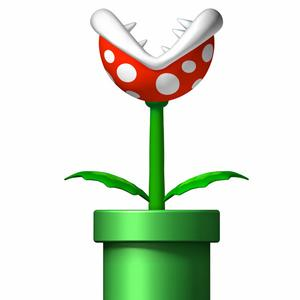
\includegraphics[width=\linewidth]{1-Theory/figs/plant}		
	\end{subfigure}
	\begin{subfigure}{.05\textwidth}%
		\vspace{-5cm}\caption{}\label{sfig:secondaty2}
		\end{subfigure}
	\begin{subfigure}{.43\textwidth} 
			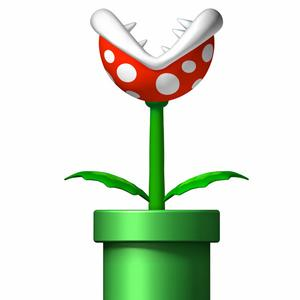
\includegraphics[width=\linewidth]{1-Theory/figs/plant}
	\end{subfigure}%
	\vspace*{-.25cm}
	\caption[Example of Figure title]{The explanation of your figures. \blindtext}	\label{fig:Main}	
	\end{figure}	
				
\Blindtext


	\section{Mie Theory: Spherical Symmetry}
%	\section{Depolarization Factors}

\chapter{Results and discussion}
	\section{Finite Element Method and Analytical Solutions}
	\section{Incrustation Degree of a Spherical Particle}
	
\chapter{Conclusions}
    \section{Future Work: Application on Metasurfaces}
        
\appendix
\chapter{The Finite Element Method}
%
%\section{Template}
%% !TeX root = ../tesis.tex

\chapter{Theory}
\label{chapter:theory}

\vspace*{7em}

It is recommended to write a summary about the contents of this chapter as an introduction to them. 

\blindtext

\section{The Basics}
\label{section:basics}

If you want to frame some equations because you consider them important, use the \textbf{tcolorbox} command. Also, you may use the \textbf{subequations} command sometimes. Fot example with the Maxwell's equations \cite{griffiths2013electrodynamics}:\vspace*{-.75em}
%
	\begin{subequations} \label{eqs:Maxwell}
	\begin{tcolorbox}[title = Ecuaciones de Maxwell en el sistema internacional de unidades,
	ams align, breakable]
	\nabla \cdot\vb{E} &= \frac{\rho_{tot}}{\varepsilon_0}, &\mbox{(Ley de Gauss eléctrica)}  
	\label{seq:GE} \\
	\nabla \cdot\vb{B} &= 0,						&\mbox{(Ley de Gauss magnética)}   
	\label{seq:GM} \\
	\nabla \times\vb{E} &= -\pdv{\vb{B}}{t}, 	&\mbox{(Ley de Faraday-Lenz)}		
	\label{seq:FL}\\
	\nabla \times\vb{B} &= \mu_0 \vb{J}_{tot} +\varepsilon_0\mu_0 \pdv{\vb{E}}{t}, &
	\mbox{(Ley de Ampère-Maxwell)} \label{seq:AM}
	\end{tcolorbox}\end{subequations}\vspace*{-.75em}\noindent
%
and if you want them to appear in the analytical index just use the \textbf{index} command \textbackslash index\{ \}.\index{Maxwell!ecuaciones de}

If you want to show two equations in only one row, use the macros \textbf{\textbackslash eqhalf}, for example\cite{hecht1998optics} \index{Ecuación!de onda}, for the Fourier transform \footnote{\setstretch{1.0} $\mathcal{F}[f(\vb{r},\omega)] = \int_{-\infty}^\infty f(\vb{r},t) e^{i(\vb{k}\cdot\vb{r} -\omega t)} dt$, con $\vb{k}$ una función de $\omega$. La transformada de Fourier inversa es entonces $\mathcal{F}^{-1}[f(\vb{r},t)] =\frac{1}{2\pi} \int_{-\infty}^\infty f(\vb{r},\omega) e^{i(\vb{k}\cdot\vb{r} -\omega t)} d\omega$.\index{Fourier! Transform}} or the Helholtz equation \index{Equation! Helmholtz} for $\vb{E}$ y $\vb{B}$ \cite{griffiths2013electrodynamics}

	\begin{subequations}%
	\eqhalf{\nabla^2\vb{E} + k^2 \vb{E}=\vb{0},}%
	\eqhalf{\nabla^2\vb{B} + k^2 \vb{B}=\vb{0}.}\label{eq:Helmholtz}%
	\end{subequations}\vspace*{-1em}

\noindent leading to plane waves as follow

	\begin{subequations}%
	\eqhalf{\vb{E}(\vb{r},t) =\vb{E_0}e^{i(\vb{k}\cdot\vb{r} -\omega t)},}%
	\eqhalf{\vb{B}(\vb{r}, t) =\vb{B_0}e^{i(\vb{k}\cdot\vb{r} -\omega t),}}	
	\label{eqs:ondasPlanas}\end{subequations}\vspace*{-1em}
		
\noindent \blindtext \vspace*{-.75em}
%
	\begin{tcolorbox}[title = Índice de refracción, ams align]
	n(\omega) = \sqrt{\frac{\mu\varepsilon(\omega)}{\varepsilon_0 \mu_0}}.
		\label{eq:indice} 
	\end{tcolorbox}\vspace*{-.75em}

For the figures, you can use this format:
%
	\begin{figure}[h!]\centering
	\begin{subfigure}{.05\textwidth}%
		\caption{}\label{sfig:secondary1}\vspace*{5cm}
	\end{subfigure}
	\begin{subfigure}{.43\textwidth} 
			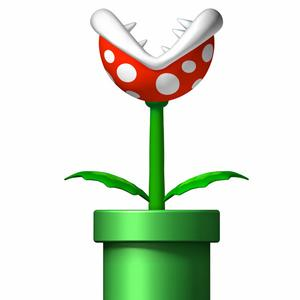
\includegraphics[width=\linewidth]{1-Theory/figs/plant}		
	\end{subfigure}
	\begin{subfigure}{.05\textwidth}%
		\vspace{-5cm}\caption{}\label{sfig:secondaty2}
		\end{subfigure}
	\begin{subfigure}{.43\textwidth} 
			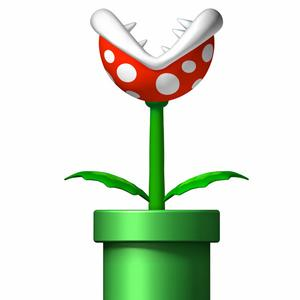
\includegraphics[width=\linewidth]{1-Theory/figs/plant}
	\end{subfigure}%
	\vspace*{-.25cm}
	\caption[Example of Figure title]{The explanation of your figures. \blindtext}	\label{fig:Main}	
	\end{figure}	
				
\Blindtext

%	% !TeX root = ../tesis.tex


\section{Somethinf more specific}
\label{section:basics}
				
\Blindtext

%% !TeX root = ../tesis.tex


\chapter{Results}

\section{What I got}
\label{section:results}
				
\Blindtext

%% !TeX root = ../tesis.tex
\chapter*{Conclusions}\addcontentsline{toc}{chapter}{\protect\numberline{}Conclusions}
\label{chapter:concl}

Make a short summary of the content of the thesis \cite{reyes2018analytical,pena-gomar2006coherent,barrera1991optical,garcia2012multiple} and then your conclusions. Also explain your future steps on this project 

\blindtext

\blindtext
        
%
%%-------------------------------------------------------------------------------
%%                               References                                   |
%%-------------------------------------------------------------------------------
%
%\appendix
%% !TeX root = ../tesis.tex


\chapter{What I couldn't get into the main part}

\label{section:apendix1}
				
\Blindtext
  

\setlength\bibitemsep{.1\itemsep}
\printbibliography

\newpage
\listoffigures

\printindex
%-------------------------------------------------------------------------------
%                              Appendix                                   |
%-------------------------------------------------------------------------------


           
\end{document}
